\newpage
\subsection{Caso d'uso UC7: Compilazione questionario selezionato}
\label{UC7}
\begin{figure}[h]
\centering
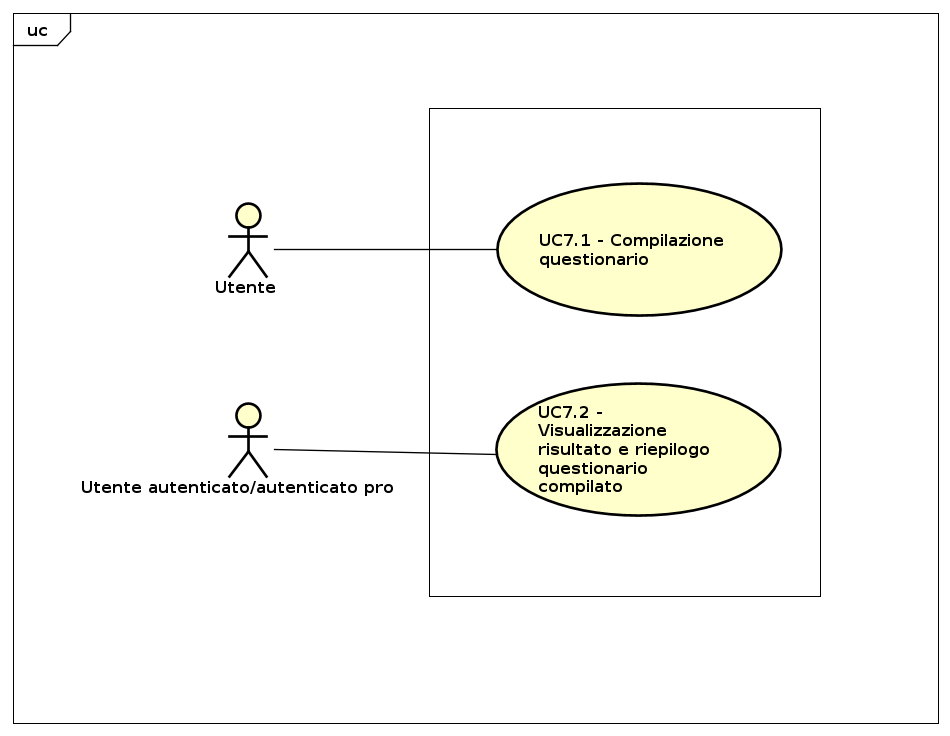
\includegraphics[scale=0.5,keepaspectratio]{UML/UC7.png}
\caption{UC7: Compilazione questionario selezionato}
\end{figure}
\FloatBarrier
\begin{itemize}
\item\textbf{Attori Principali}: Utente non autenticato, Utente autenticato, Utente autenticato pro;
\item\textbf{Descrizione}: l'utente autenticato/autenticato pro può compilare qualsiasi tipo di questionario e infine visualizzare il risultato ottenuto e il riepilogo delle risposte date. L'utente non autenticato invece può soltanto svolgere i questionari \textit{pubblici};
\item\textbf{Precondizione}: l'utente ha selezionato un questionario;
\item\textbf{Postcondizione}: l'utente ha finito di compilare il questionario e può quindi visualizzare la valutazione finale che ha ottenuto e il riepilogo delle risposte date, se è un utente autenticato/autenticato pro;
\item\textbf{Scenario principale}:
\begin{itemize}
\item L'utente compila un questionario (UC7.1);
\item L'utente autenticato/autenticato pro visualizza il risultato e il riepilogo del questionario svolto (UC7.2).
\end{itemize}
\item\textbf{Scenari alternativi}: l'utente non vuole più compilare il questionario e annulla così questa operazione tornando alla schermata principale.
\end{itemize}

\subsubsection{Caso d'uso UC7.1: Compilazione questionario}
\label{UC7.1}
\begin{figure}[h]
\centering
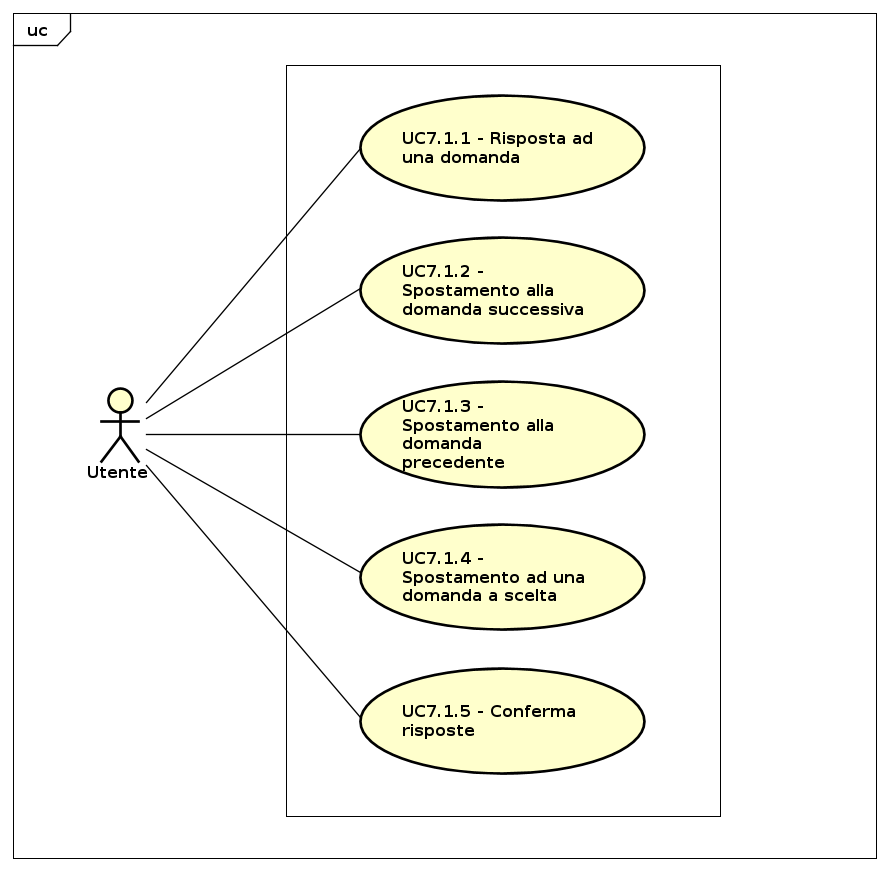
\includegraphics[scale=0.5,keepaspectratio]{UML/UC7_1.png}
\caption{UC7.1: Compilazione questionario}
\end{figure}
\FloatBarrier
\begin{itemize}
\item\textbf{Attori Principali}: Utente non autenticato, Utente autenticato, Utente autenticato pro;
\item\textbf{Descrizione}: l'utente può rispondere alle domande che gli si presentano nell'ordine che preferisce spostandosi alla domanda successiva, a quella precedente oppure ad una a sua scelta e infine conferma le risposte date;
\item\textbf{Precondizione}: l'utente ha selezionato un questionario;
\item\textbf{Postcondizione}: l'utente ha compilato il questionario;
\item\textbf{Scenario principale}:
\begin{itemize}
\item L'utente risponde ad una domanda (UC7.1.1);
\item L'utente passa alla domanda successiva (UC7.1.2);
\item L'utente passa alla domanda precedente (UC7.1.3);
\item L'utente passa ad una domanda a sua scelta (UC7.1.4);
\item L'utente conferma le risposte date alle domande (UC7.1.5).
\end{itemize}
\end{itemize}

\subsubsection{Caso d'uso UC7.1.1: Risposta ad una domanda}
\label{UC7.1.1}
\begin{figure}[h]
\centering
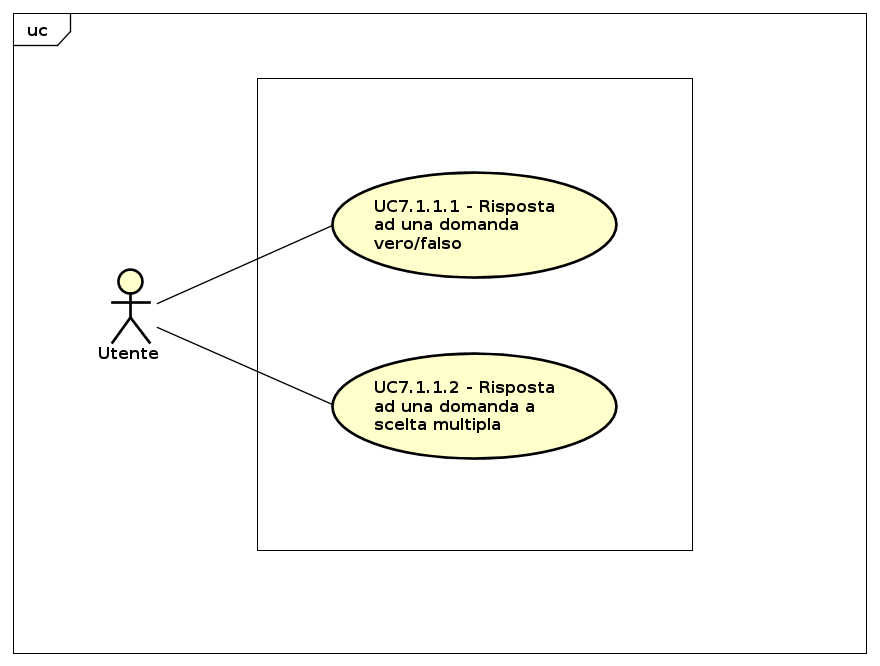
\includegraphics[scale=0.5,keepaspectratio]{UML/UC7_1_1.png}
\caption{UC7.1.1: Risposta ad una domanda}
\end{figure}
\FloatBarrier
\begin{itemize}
\item\textbf{Attori Principali}: Utente non autenticato, Utente autenticato, Utente autenticato pro;
\item\textbf{Descrizione}: l'utente può rispondere, una alla volta, alle varie domande che compongono il questionario che possono essere di due tipi:
\begin{itemize}
\item Vero/falso;
\item Scelta multipla.
\end{itemize}
\item\textbf{Precondizione}: l'utente sta compilando un questionario;
\item\textbf{Postcondizione}: l'utente ha selezionato una risposta;
\item\textbf{Scenario principale}: 
\begin{itemize}
\item L'utente risponde ad una domanda vero/falso (UC7.1.1.1);
\item L'utente risponde ad una domanda a scelta multipla (UC7.1.1.2).
\end{itemize}
\end{itemize}

\subsubsection{Caso d'uso UC7.1.1.1: Risposta ad una domanda vero/falso}
\label{UC7.1.1.1}
\begin{itemize}
\item\textbf{Attori Principali}: Utente non autenticato, Utente autenticato, Utente autenticato pro;
\item\textbf{Descrizione}: l'utente può rispondere ad una domanda vero/falso selezionando una delle due alternative;
\item\textbf{Precondizione}: l'utente sta compilando un questionario;
\item\textbf{Postcondizione}: l'utente ha selezionato una risposta;
\item\textbf{Scenario principale}: l'utente seleziona una risposta tra vero e falso.
\end{itemize}

\subsubsection{Caso d'uso UC7.1.1.2: Risposta ad una domanda a scelta multipla}
\label{UC7.1.1.2}
\begin{itemize}
\item\textbf{Attori Principali}: Utente non autenticato, Utente autenticato, Utente autenticato pro;
\item\textbf{Descrizione}: l'utente può rispondere ad una domanda a scelta multipla selezionando una delle quattro alternative;
\item\textbf{Precondizione}: l'utente sta compilando un questionario;
\item\textbf{Postcondizione}: l'utente ha selezionato una risposta;
\item\textbf{Scenario principale}: l'utente seleziona una risposta tra le quattro proposte.
\end{itemize}

\subsubsection{Caso d'uso UC7.1.2: Spostamento alla domanda successiva}
\label{UC7.1.2}
\begin{itemize}
\item\textbf{Attori Principali}: Utente non autenticato, Utente autenticato, Utente autenticato pro;
\item\textbf{Descrizione}: l'utente può passare alla domanda successiva;
\item\textbf{Precondizione}: l'utente sta compilando un questionario;
\item\textbf{Postcondizione}: il sistema visualizza la domanda successiva;
\item\textbf{Scenario principale}: l'utente seleziona il comando per passare alla domanda successiva.
\end{itemize}

\subsubsection{Caso d'uso UC7.1.3: Spostamento alla domanda precedente}
\label{UC7.1.3}
\begin{itemize}
\item\textbf{Attori Principali}: Utente non autenticato, Utente autenticato, Utente autenticato pro;
\item\textbf{Descrizione}: l'utente può passare alla domanda precedente;
\item\textbf{Precondizione}: l'utente sta compilando un questionario;
\item\textbf{Postcondizione}: il sistema visualizza la domanda precedente;
\item\textbf{Scenario principale}: l'utente seleziona il comando per passare alla domanda precedente.
\end{itemize}

\subsubsection{Caso d'uso UC7.1.4: Spostamento ad una domanda a scelta}
\label{UC7.1.4}
\begin{itemize}
\item\textbf{Attori Principali}: Utente non autenticato, Utente autenticato, Utente autenticato pro;
\item\textbf{Descrizione}: l'utente può passare ad una domanda a sua scelta selezionandola attraverso la tabella delle domande. Queste saranno identificate da un numero, in base all'ordine in cui sono poste all'interno del questionario, e da un colore, arancioni se è già stata data una risposta oppure grige in caso contrario;
\item\textbf{Precondizione}: l'utente sta compilando un questionario;
\item\textbf{Postcondizione}: il sistema visualizza la domanda selezionata dall'utente;
\item\textbf{Scenario principale}: l'utente seleziona una domanda a cui deve ancora rispondere o una alla quale vuole cambiare la risposta data.
\end{itemize}

\subsubsection{Caso d'uso UC7.1.5: Conferma risposte}
\label{UC7.1.5}
\begin{itemize}
\item\textbf{Attori Principali}: Utente non autenticato, Utente autenticato, Utente autenticato pro;
\item\textbf{Descrizione}: l'utente può confermare le domande a cui ha dato una risposta;
\item\textbf{Precondizione}: l'utente sta compilando un questionario;
\item\textbf{Postcondizione}: l'utente ha confermato le risposte date;
\item\textbf{Scenario principale}: l'utente che ha finito di rispondere a tutte le domande conferma le risposte date;
\item\textbf{Scenari alternativi}: l'utente conferma le risposte date anche se non le ha compilate tutte, accettando il fatto che queste verranno considerate sbagliate.
\end{itemize}

\subsubsection{Caso d'uso UC7.2: Visualizzazione risultato e riepilogo questionario compilato}
\label{UC7.2}
\begin{itemize}
\item\textbf{Attori Principali}: Utente autenticato, Utente autenticato pro;
\item\textbf{Descrizione}: l'utente, dopo aver finito di compilare il questionario, può visualizzare una schermata contenente il riepilogo delle risposte date alle domande. Sarà possibile vedere quali di queste sono corrette e quali no e verrà inoltre data una valutazione complessiva;
\item\textbf{Precondizione}: l'utente ha finito di compilare il questionario che ha scelto di affrontare;
\item\textbf{Postcondizione}: il sistema visualizza una schermata contenente il riepilogo del questionario svolto e un voto;
\item\textbf{Scenario principale}: l'utente visualizza che voto gli è stato dato e quali domande ha sbagliato.
\end{itemize}

